\documentclass[12pt,onecolumn]{report}
\usepackage[T1]{fontenc}
\usepackage[utf8]{inputenc}
\usepackage[francais]{babel}
\usepackage{amsfonts,amsmath,amssymb}
\usepackage{graphicx}
\usepackage{tikz}

\begin{document} 
\begin{figure}
	\begin{flushleft}
        
\includegraphics[width=0.2\linewidth]{POLYTECHNIQUE-IP_PARIS}
        \hspace{6.6cm}
        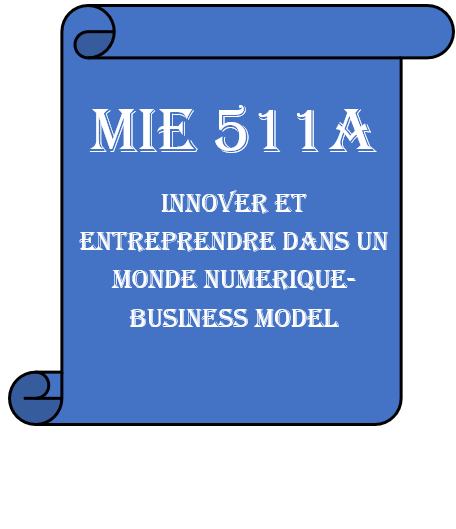
\includegraphics[width=0.3\linewidth]{14}
	\end{flushleft}
 \vspace{2.7cm}
\end{figure}   
    \begin{center}
    	INSTITUT POLYTECHNIQUE DE PARIS\\
    	COUR MIE511A:INNOVER ET ENTREPRENDRE DANS UN MONDE NUMERIQUE-BUSINESS MODEL.\\[0.8cm]
    	Professeur: THIERRY RAYNA\\[0.8cm]
    	\textbf{Thème du 03/10/2019:}Dans un secteur d'activité de votre choix, identifiez des activités d'open innovation ou de co-création. Quels problèmes ces activités visent elles à surmonter?.\\[0.5cm]
    	\textbf{Sujet:}Open innovation et co-création dans le secteur de la défense..\\[1cm]
    \end{center}
	\begin{flushleft}
		    Etudiant:Elise Al Neimi\\
			Etudiant:Panongbene Jean Mouhamed Sawadogo.\\
			Etudiant:Thomas Simonneau\\
			Etudiant:Mohammed El Mendili
	\end{flushleft}
	\begin{tikzpicture}
		\draw (0,1) -- (0,10); 
		\draw (2,2) -- (0,4);
	\end{tikzpicture}
\thispagestyle{empty}
\setcounter{page}{0}
\newpage
\begin{center}
	\centering{\textbf{SOMMAIRE:}}
\end{center}
\MakeUppercase{\romannumeral 1}. INTRODUCTION\\[0.2cm]
\MakeUppercase{\romannumeral 2}. OUTSIDE-IN : EXEMPLE DU FLYBOARD AIR.\\[0.2cm]
\MakeUppercase{\romannumeral 3}. INSIDE-OUT : EXEMPLE DES DRONES.\\[0.2cm]
\MakeUppercase{\romannumeral 4}. MANQUE DE MOYENS \& D'EXPERTISE : EXEMPLE DE PALANTIR.\\[0.2cm]
\MakeUppercase{\romannumeral 5}. CONCLUSION\\

\end{document}